\documentclass[12pt,a4paper]{report}

\usepackage{etoolbox}% http://ctan.org/pkg/etoolbox

\usepackage{lmodern} % add the missing package for font shapes
\usepackage[]{qcircuit}

\renewcommand\familydefault{\sfdefault} % sans serif

\usepackage[margin=2.54cm]{geometry}	% dimensiuni pagină și margini
\usepackage{graphicx} % support the \includegraphics command and options

% formatting sections and subsections
\usepackage{textcase}
\usepackage[titletoc, title]{appendix}
\usepackage{titlesec}
\titleformat{\chapter}{\large\bfseries\MakeUppercase}{\thechapter}{3ex}{}[\vspace*{-1.5cm}]
\titleformat*{\section}{\large\bfseries}
\titleformat*{\subsection}{\large\bfseries}
\titleformat*{\subsubsection}{\large\bfseries}

\usepackage{chngcntr}
\counterwithout{figure}{chapter} % no chapter number in figure labels
\counterwithout{table}{chapter} % no chapter number in table labels
\counterwithout{equation}{chapter} % no chapter number in equation labels

\usepackage{booktabs} % for much better looking tables
\usepackage{url} % Useful for inserting web links nicely
\usepackage[bookmarks,unicode,hidelinks]{hyperref}

\usepackage{array} % for better arrays (eg matrices) in maths
\usepackage{paralist} % very flexible & customisable lists (eg. enumerate/itemize, etc.)
\usepackage{verbatim} % adds environment for commenting out blocks of text & for better verbatim
\usepackage{subfig} % make it possible to include more than one captioned figure/table in a single float
\usepackage{enumitem}
\setlist{noitemsep}

%%% HEADERS & FOOTERS
\usepackage{fancyhdr}
\pagestyle{empty}
\renewcommand{\headrulewidth}{0pt}
\renewcommand{\footrulewidth}{0pt}
\lhead{}\chead{}\rhead{}
\lfoot{}\cfoot{\thepage}\rfoot{}



\newcommand{\HeaderLineSpace}{-0.25cm}
\newcommand{\UniTextEN}{POLYTECHNIC UNIVERSITY OF BUCHAREST \\[\HeaderLineSpace]
FACULTY OF AUTOMATIC CONTROL AND COMPUTERS \\[\HeaderLineSpace]
COMPUTER SCIENCE AND ENGINEERING DEPARTMENT\\}
\newcommand{\DiplomaEN}{BACHELOR THESIS}
\newcommand{\AdvisorEN}{Thesis advisor:}
\newcommand{\BucEN}{BUCHAREST}

\newcommand{\frontPage}[6]{
\begin{titlepage}
\begin{center}
{\Large #1}  % header (university, faculty, department)
\vspace{50pt}
\begin{tabular}{p{4.15cm}p{6cm}p{4.15cm}}
\vspace{-1pt}

\includegraphics[scale=0.12]{pics/upb.png} &
\vspace{-6.5pt}
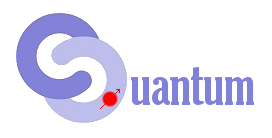
\includegraphics[scale=0.6]{pics/LogoIQC.png} &
\vspace{-2pt}

\includegraphics[scale=0.22]{pics/cs.png}
\end{tabular}

\vspace{75pt}
{\Huge #2}\\                           % diploma project text
\vspace{40pt}
{\Large #3}\\ \vspace{25pt}  % project title
{\Large #4}\\                          % project subtitle
\vspace{40pt}
{\LARGE \Name}\\                   % student name
\end{center}
\vspace{60pt}
\begin{tabular*}{\textwidth}{@{\extracolsep{\fill}}p{6cm}r}
&{\large\textbf{#5}}\vspace{10pt}\\      % scientific advisor
&{\large \Advisor}                                    % advisor name
\end{tabular*}
\vspace{20pt}
\begin{center}
{\large\textbf{#6}}\\                                % bucharest
\vspace{0pt}
{\normalsize \Year}
\end{center}
\end{titlepage}
}

\newcommand{\frontPageEN}{\frontPage{\UniTextEN}{\DiplomaEN}{\ProjectTitleEN}{\ProjectSubtitleEN}{\AdvisorEN}{\BucEN}}

\linespread{1.1}
\setlength\parindent{0pt}
\setlength\parskip{.23cm}

%% Abstract macro
\newcommand{\AbstractPage}{
\begin{titlepage}
{\large \textbf{ABSTRACT}}\vspace{10pt}\\
\AbstractEN \vfill
\end{titlepage}
}

%% Thank you macro
\newcommand{\ThanksPage}{
\begin{titlepage}
{\large \textbf{ACKNOWLEDGEMENTS}}\vspace{10pt}\\
\Thanks \vfill
\end{titlepage}
}



%%%%%%%%%%%%%%%%%%%%%%%%%%%%%%%%%%%%%%%%%%%%%%%%%%   
%%
%%          End of template definitions
%%   
%%%%%%%%%%%%%%%%%%%%%%%%%%%%%%%%%%%%%%%%%%%%%%%%%%


%%% Puteți elimina aceste linii din lucrare, servesc numai pentru template.
\newcommand{\worktype}[1]{[\textit{#1}] }
\newcommand{\dezvoltare}{\worktype{Dezvoltare de produs}}
\newcommand{\cercetare}{\worktype{Cercetare}}
\newcommand{\ambele}{\worktype{Ambele}}
%%%


%%
%%   Campurile de mai jos trebuie modificate de autor. Modificati doar continutul, nu si numele fiecarei definitii
%%
\newcommand{\ProjectTitleEN}{Investigations into Quantum Physics Integration in Deep Learning Models for Computer Vision and Natural Language Processing Fields}
\newcommand{\ProjectSubtitleEN}{QRKT-GAN: Neural Ordinary Differential Equation Generative Adversarial Network Model with Runge-Kutta Methods for Quantum Visual Transformer-Based Generator and Discriminator}
\newcommand{\Name}{Cătălin-Alexandru Rîpanu}
\newcommand{\Advisor}{Șl. dr. ing. Dumitru-Clementin Cercel}
\newcommand{\Year}{2024}

% Setări document
\title{Diploma Project}
\author{\Name}
\date{\Year}

%%
%%   Campurile aferente rezumatului
%%

\newcommand{\AbstractEN}{Deep learning models, such as Generative Adversarial Networks (GANs)~\cite{goodfellow2014generative} and Visual Transformers (ViTs)~\cite{vaswani2017attention}, have demonstrated remarkable results across various domains in Machine Learning and Artificial Intelligence, including Object Classification, Image Segmentation, Sentiment Analysis, and Machine Translation. These models are pivotal in advancing systems that require high precision and a deep understanding of complex data across a variety of tasks in both Natural Language Processing (NLP) and Computer Vision (CV).

However, the effectiveness of deep learning models comes with significant challenges: they require an extensive number of parameters to learn and extract meaningful features from real-world data. Additionally, these models need vast amounts of information to achieve desired performance levels. Obtaining such large sets can be difficult as real-world data is often not publicly available and can be challenging to collect and curate. This results in substantial computational resource requirements for both training and hyperparameter optimization, often achieved through exhaustive techniques such as grid search.

To address these challenges, this thesis proposes a novel hybrid Generative Adversarial Network architecture that employs Quantum Visual Transformers (QViTs) as both the Generator and Discriminator. Visual Transformers are selected for their superior ability to manage intricate data representations. A key innovation in this architecture is the integration of Ordinary Differential Equation (ODE)~\cite{fan2024quantum} solvers as Encoders, enhancing the model's capability to capture temporal dynamics and complex data structures, and improving the residual connections within the transformer architecture to mitigate the vanishing gradients problem even more.

Moreover, this architecture incorporates Variational Quantum Circuits~\cite{cerezo2021variational} within both the self-attention mechanisms and the Multi-Layer Perceptrons (MLPs)~\cite{popescu2009multilayer} of the Visual Transformers. By leveraging the principles of quantum mechanics, these quantum circuits can perform complex algebraic operations more efficiently than classical methods, offering a significant computational advantage.

The performance of this hybrid model is benchmarked against SoTA purely classical baselines from the literature using datasets from both CV and NLP areas. Specifically, the model is tested on CIFAR-10~\cite{Krizhevsky09learningmultiple}, CIFAR-100~\cite{Krizhevsky09learningmultiple}, MNIST~\cite{lecun2010mnist}, IMDb Reviews~\cite{maas-EtAl:2011:ACL-HLT2011} and ImageNet(2012)~\cite{ILSVRC15}  datasets. The quantum model is successfully trained and tested through numerical simulations. The results indicate that this hybrid approach achieves comparable classification and generation performance to the classical baseline, while requiring fewer trainable parameters.

Furthermore, the reduced parameter count in this hybrid model opens up the possibility of running it on real quantum hardware for both training and inference. This feasibility is a significant breakthrough, as it implies that quantum-enhanced models can be trained and deployed on actual quantum computers, which are currently limited in terms of the number of qubits and operational fidelity.

This thesis demonstrates the potential of integrating quantum computing, especially quantum mechanics, with advanced deep learning architectures to create more efficient and powerful networks which can significantly reduce computational costs while maintaining high performance, paving the way for more scalable and effective AI applications.}

%%
%%   Campurile aferente paginii de multumiri
%%
\newcommand{\Thanks}{
First and foremost, I would like to express my deepest gratitude to my advisor, Prof. Dumitru-Clementin Cercel, for his unwavering support and insightful guidance throughout my research journey. His expertise and encouragement have been essential in exploring the intricate intersection of Artificial Intelligence and Quantum Mechanics, widely referred to in the literature as Quantum Artificial Intelligence. This interdisciplinary field, though initially daunting, is at the cutting edge of technological advancement and innovation in both areas.

I am also profoundly thankful to Prof. Pantelimon-George Popescu for his advice, recommendations, and exceptional lectures on Quantum Computing. His mentorship has been instrumental in building a robust understanding of this groundbreaking paradigm, which promises new solutions to problems previously deemed insurmountable by classical methods.

Furthermore, I wish to acknowledge the significant contributions of the academic teaching assistants and collaborators encountered during my bachelor's studies. Their guidance during challenging times has been crucial to my academic development. Last but not least, I am also grateful for the computational resources provided by the Computer Science and Engineering Department, which were essential for the design and implementation of this project.

In addition, I extend my appreciation to my friends for their continuous support, ideas, and advice, especially during moments when inspiration was scarce. Lastly, my heartfelt thanks go to my parents for their enduring sacrifices and unwavering support throughout this journey into the unknown. Their belief in me has been a constant source of motivation.
}

\makeatletter
\def\@makechapterhead#1{%
  \vspace*{-25\p@}%
  {\parindent \z@ \raggedright \normalfont
  \ifnum \c@secnumdepth >\m@ne
  \Large\bfseries \thechapter\space% Adjust the size as needed
  \fi
  \interlinepenalty\@M
  \Large \bfseries #1\par\nobreak
  \vskip 11\p@
  }}
  
\makeatother

\begin{document}

\setcounter{page}{1}
\frontPageEN

\setcounter{page}{2}
\ThanksPage \pagestyle{fancy}

\AbstractPage\pagestyle{fancy}

\renewcommand{\contentsname}{\vspace{-2.35cm} CONTENTS}
\tableofcontents
% Textul licentei incepe de aici 

\chapter{Introduction}\pagestyle{fancy}

\section{Context}\vspace{-15pt}
Artificial Intelligence models, particularly deep learning ones, have made significant contributions to solving real-world tasks, greatly improving human lives in various fields, such as Medical Disease Recognition. Despite their impressive capabilities, deep learning models come with substantial drawbacks regarding computational resources and effort. Achieving high performance with these models necessitates learning millions to billions of parameters (also called weights or artificial neurons), which demands considerable resources and preparation time. This limitation also has negative environmental impacts due to high power consumption.

Over the years, researchers have developed numerous solutions to mitigate the problem of minimizing the number of parameters using interesting classical algorithms and techniques. These include specialized activation functions for layers like Rectified Linear Unit~\cite{NIPS2017_a96b65a7}, Leaky ReLU~\cite{xu2020reluplex}, Gaussian Error Linear Unit~\cite{hendrycks2016gaussian}, Softmax~\cite{liu2016large}, Sigmoid~\cite{han1995influence} and Hyperbolic Tangent~\cite{zamanlooy2013efficient}. Additionally, effective optimizers such as Adam~\cite{zhang2018improved} and Stochastic Gradient Descent~\cite{bottou2010large} have been utilized, along with Learning Rate Schedulers~\cite{wen2021convolutional}, Weight Decay~\cite{loshchilov2017decoupled}, and Dropout~\cite{srivastava2014dropout} methods to combat overfitting too. Over the years, various architectural designs and network combinations have emerged to address these challenges. However, the tradeoff between high computational resource consumption and performance remains a difficult issue, especially when scaling up the dimensions of available noisy real-world datasets used for training. It is unlikely to be efficiently resolved in the near future using solely classical approaches.

A segment of Computer Science researchers, in collaboration with physicists, have taken a bold and innovative approach to these challenges by exploring solutions from a physical perspective, leading to the emergence of Quantum Computation and Quantum Information~\cite{nielsen2001quantum}. Leveraging the principles of quantum mechanics, AI research has begun to explore deep learning optimizations using quantum elements, such as Variational Quantum Circuits~\cite{cerezo2021variational}, to develop hybrid deep learning models. By combining classical and quantum methodologies, new experiments can be conducted to address performance and resource demands more efficiently, thus utilizing the unique capabilities of quantum hardware. This involves training these models on it, also known as Parameterized Quantum Circuits, where the parameters are referred to as qurons of the quantum model.

Quantum computing leverages properties like superposition and entanglement, enabling the execution of complex algebraic operations that are infeasible for classical computers. Quantum algorithms, such as Grover's Algorithm~\cite{shi2017coherence}, Quantum Phase Estimation~\cite{o2019quantum}, Quantum Fourier Transform~\cite{weinstein2001implementation} and Deutsch-Jozsa Quantum Parallelism~\cite{gulde2003implementation} provide exponential speedups for certain tasks. Integrating these quantum principles with deep learning can significantly reduce the number of parameters and computational resources required while maintaining or even enhancing model performance. This interdisciplinary approach, also known as Quantum Artificial Intelligence, opens up exciting possibilities for the future of AI, promising advancements that could transform how complex problems are approached and solved in ways that classical computers, with their current architecture, could never achieve.
\section{Problem}\vspace{-15pt}
Over the years, numerous algorithms, techniques, network architectures, and methodologies have been proposed in the field of Deep Learning to tackle a wide array of tasks, such as Object Classification, Synthetic Data Generation and Detection, across various domains including Natural Language Processing, Computer Vision, Domain Adaptation, and Knowledge Distillation. These approaches have achieved high performance metrics like accuracy, Area Under the Curve (AUC), Receiver Operating Characteristic (ROC), and F1 scores. The advent of High Performance Computing (HPC) facilities, particularly classical parallelism, has enabled deep learning models to process billions of examples from noisy real-world datasets effectively, thus yielding impressive results.

Despite these advancements, a significant drawback persists: the enormous number of neurons and the corresponding computational resources required by these models. Traditional solutions in classical Deep Learning, such as Cross Validation~\cite{berrar2019cross}, Hyperparameter Tuning techniques like Grid Search~\cite{liashchynskyi2019grid}, Random Search~\cite{liashchynskyi2019grid}, or Keras Tuner~\cite{pon2021hyperparameter}, and Layer Augmentation until model performance plateaus or overfits, are commonly employed. To mitigate overfitting, regularization techniques such as Ridge~\cite{ogutu2012genomic}, Lasso~\cite{ogutu2012genomic} or Elastic-Net~\cite{ogutu2012genomic} Regularizations, or Dropout~\cite{srivastava2014dropout} can be applied. However, these methods often involve exhaustive hyperparameter searches, which are extremely time-consuming, especially when dealing with validation sets comprising billions of data points for complex tasks. Additionally, one can apply group sparsity regularizers on network parameters, where each group acts on a single neuron, thus reducing the number of parameters by up to 80\%~\cite{alvarez2018learning} while retaining or even improving the network accuracy.

Another method employed to address these challenges is Transfer Learning, which involves finding and loading a pretrained model as a starting point and then fine-tuning it on a specific dataset. This approach can help achieve good performance with less effort on architecture design and expedite the training process. However, the availability of suitable pretrained models is limited, and fine-tuning may yield only decent, if not disappointing, results, due to differences in the data distributions between the pretraining and fine-tuning datasets.

The primary challenge lies in balancing time and power consumption on classical systems to make non-trivial, valid neural architectural choices. Reducing the number of neurons too drastically can lead to underfitting and degraded performance, making it difficult to solve complex and challenging tasks efficiently. The iterative process of tuning hyperparameters and optimizing model architectures is computationally intensive and often results in a significant trade-off between resource consumption and model performance.

Moreover, the reliance on vast amounts of training data for achieving desired performance further exacerbates these issues. Real-world data is often difficult to obtain and may not be publicly available, which complicates the development and fine-tuning of effective deep learning models. The extensive time and computational costs associated with hyperparameter optimization and model training present significant obstacles to advancing AI capabilities while maintaining efficiency and sustainability. This trade-off between computational resource consumption and performance remains a persistent and challenging problem in the field of deep learning, highlighting the need for innovative solutions that can overcome these limitations.

\section{Objective}\vspace{-15pt}
In the current landscape of deep learning research, there is an ongoing investigation into whether integrating models into a purely quantum environment can significantly reduce power consumption and the number of trainable parameters without sacrificing performance. This exploration leverages techniques such as Ansatz~\cite{hadfield2019quantum} and Variational Quantum Circuits~\cite{cerezo2021variational}. As classical supercomputers continue to increase in power to accommodate newer, more complex deep models, their power consumption scales almost exponentially. Conversely, while the computational power of quantum machines scales exponentially, their power consumption scales linearly. This presents a compelling argument for quantum computing: when quantum computers achieve fault-tolerance, operations on qubits could serve as artificial neurons in neural networks. Quantum-inspired techniques could enable networks with a vast number of neurons per layer to run with minimal energy cost, thus dramatically reducing overall energy consumption\footnote{\url{https://www.eetimes.eu/how-quantum-computing-can-help-make-ai-greener/}}.

Building on the challenges outlined in the above section, the primary goal of this thesis is to explore deep learning models, both pure quantum and hybrid, that leverage neural architectures inspired by non-trivial Variational Quantum Circuits~\cite{cerezo2021variational} within the context of Visual Transformers~\cite{vaswani2017attention} and their Encoders~\cite{hinton2011transforming} and Decoders~\cite{breuckmann2018scalable}. The most important objective is to minimize the number of parameters used by deep network layers utilizing the idea of replacing classical linear projection layers in Multi-Head Attention subroutines and Multi-Layer Perceptrons~\cite{popescu2009multilayer} with Quantum Circuits. Additionally, Neural Ordinary Differential Equation~\cite{zhong2022neural}\cite{li2022ode} techniques, particularly using Runge-Kutta Methods~\cite{butcher1996history} of 1st, 2nd, 3rd, and 4th order, will be employed to further optimize Transformer Layers. An analysis of 4th order optimization in terms of learning efficiency will also be included.

These configurations will be rigorously tested using the datasets mentioned in the Abstract and compared with their classical baseline counterparts. The model utilizing the Runge-Kutta 4th order method will be further optimized within the context of Vision Transformers (ViTs) and integrated into a Generative Adversarial Network (GAN) architecture. In this configuration, both the Generator and Discriminator will be Quantum Visual Transformers, incorporating the optimized Neural ODE to generate realistic and informative synthetic data without being limited to specific types of distributions. This will be achieved using techniques such as data augmentation and image recognition at scale in the context of ViTs.

The final proposed architecture, named QRKT-GAN, will be tested on a voluminous dataset, namely ImageNet (2012), and compared using the same data with a renowned classical counterpart, TransGAN, which is a strong architecture built entirely free of convolutions (citation here). This comparative analysis will highlight the efficiency and performance gains of integrating quantum computing with advanced deep learning models.
\section{Paper Structure}\vspace{-15pt}
This is the structure of the paper

\chapter{Related Work}\pagestyle{fancy}

\chapter{Background}\pagestyle{fancy}

\chapter{Proposed Solution}\pagestyle{fancy}

\chapter{Experiments}\pagestyle{fancy}

\chapter{Conclusions and Future Work}\pagestyle{fancy}

\chapter{Bibliography}\pagestyle{fancy}

\bibliographystyle{unsrt}

\begingroup
\def\chapter*#1{}
\bibliography{bibliography}
\endgroup

\end{document}
